\section{Related Research\label{sec:related-work}}
  FRNNs searches are most often found within agent-based models, they have also been used alongside similar algorithms within the fields of \gls{sph} and collision detection. FRNNs is the process whereby each agent considers the properties of every other agent located within a radial area about their location. This searched area can be considered the agent’s neighbourhood and must be searched every timestep of a simulation to ensure agents have live information. Whilst various spatial data-structures such as kd-trees and R-trees are capable of providing efficient access to spatial neighbourhoods, their expensive constructions however, make them unsuitable for the large dynamic agent populations found within agent-based models.

  The naive technique for carrying out a neighbourhood search is via a brute-force technique, individually considering whether each agent is located within the target neighbourhood. This technique may be suitable for small agent populations, however the overhead quickly becomes significant as agent populations increase, reducing the proportional size of the neighbourhoods.
\begin{wrapfigure}{r}{0.5\textwidth}
  \begin{center}
    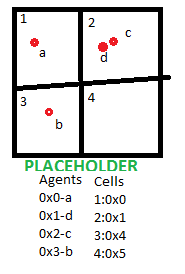
\includegraphics[width=0.48\textwidth]{../resources/USP-placeholder.png}
  \end{center}
  \caption{\label{fig:usp} A representation of the data structure used by uniform spatial partitioning.}
\end{wrapfigure}
  
  The most common technique that is used to reduce the overhead of FRNNs handling is that of uniform spatial partitioning (Figure \ref{fig:usp}), whereby the environment is partitioned into a uniform grid. Agents are then (sorted and) stored according to the ID of their containing cell within the grid. A separate index is then produced, providing fast access the storage of each cell’s agents. This allows the Moore neighbourhood of an agent’s cell to be accessed, ignoring agents within cells outside of the desired neighbourhood. This method is particularly suitable for parallel implementations\cite{Gre10} and several advances have been suggested to further improve the performance\cite{GS*10,Hoe14,HY*15}.

  Recent FRNNs publications have either provided no comparative performance results, or simply compared with an iteration lacking the published innovation\cite{GS*10,Hoe14,HY*15}. With numerous potential innovations which may interact and overlap it becomes necessary to standardise the methodology by which these advances can be compared both independently and in combination. When assessing the performance of \gls{hpc} algorithms there are various approaches which must be taken and considered to ensure fair results.
  
  When comparing the performance of algorithms there are a plethora of recommendations to be followed to ensure that results are not misleading\cite{Bai92}. The general trend among these guidelines is the requirement of explicit detailing of experimental conditions, ensuring uniformity between test cases such that results can be reproduced. Furthermore if comparing algorithm performance across different architectures it is important to ensure that appropriate optimisations for each architecture have been carried out and that the cost of relevant hardware is considered when discussing results. Historically there have been numerous cases whereby comparisons between \gls{cpu} and \gls{gpu} have shown speedups as high as 100x which have later been debunked due to flawed methodology\cite{LK*10}.

  %Microbenchmarking is also found within the \gls{hpc} community. High precision timings are collected of the repeated execution of a single operation, exposing execution costs of individual instructions and cache accesses. This work has been carried out surveying \glspl{gpu} by both Wong et al\cite{WP*10}; and Volkov and Demel\cite{VD08}, similarly Liu et al have used microbenchmarking to compare the performance within compute clusters\cite{LC*04}. Microbenchmarking primarily provides a greater understanding of architectural timings, however the lessons learned can be applied when designing \gls{hpc} algorithms. This does however make microbenchmarking unsuitable for comparing the implementations presented within this paper.